% This is based on "sig-alternate.tex" V1.9 April 2009
% This file should be compiled with V2.4 of "sig-alternate.cls" April 2009
%
\documentclass{report}

\usepackage[english]{babel}
\usepackage{graphicx}
\usepackage{tabularx}
\usepackage{subfigure}
\usepackage{enumitem}
\usepackage{url}
\usepackage{listings}
\usepackage{hyperref}


\usepackage{color}
\definecolor{orange}{rgb}{1,0.5,0}
\definecolor{lightgray}{rgb}{.9,.9,.9}
\definecolor{java_keyword}{rgb}{0.37, 0.08, 0.25}
\definecolor{java_string}{rgb}{0.06, 0.10, 0.98}
\definecolor{java_comment}{rgb}{0.12, 0.38, 0.18}
\definecolor{java_doc}{rgb}{0.25,0.35,0.75}

% code listings

\usepackage{listings}
\lstloadlanguages{Java}
\lstset{
	language=Java,
	basicstyle=\scriptsize\ttfamily,
	backgroundcolor=\color{lightgray},
	keywordstyle=\color{java_keyword}\bfseries,
	stringstyle=\color{java_string},
	commentstyle=\color{java_comment},
	morecomment=[s][\color{java_doc}]{/**}{*/},
	tabsize=2,
	showtabs=false,
	extendedchars=true,
	showstringspaces=false,
	showspaces=false,
	breaklines=true,
	numbers=left,
	numberstyle=\tiny,
	numbersep=6pt,
	xleftmargin=3pt,
	xrightmargin=3pt,
	framexleftmargin=3pt,
	framexrightmargin=3pt,
	captionpos=b
}

% Disable single lines at the start of a paragraph (Schusterjungen)

\clubpenalty = 10000

% Disable single lines at the end of a paragraph (Hurenkinder)

\widowpenalty = 10000
\displaywidowpenalty = 10000
 
% allows for colored, easy-to-find todos

\newcommand{\todo}[1]{\textsf{\textbf{\textcolor{orange}{[[#1]]}}}}

% consistent references: use these instead of \label and \ref

\newcommand{\lsec}[1]{\label{sec:#1}}
\newcommand{\lssec}[1]{\label{ssec:#1}}
\newcommand{\lfig}[1]{\label{fig:#1}}
\newcommand{\ltab}[1]{\label{tab:#1}}
\newcommand{\rsec}[1]{Section~\ref{sec:#1}}
\newcommand{\rssec}[1]{Section~\ref{ssec:#1}}
\newcommand{\rfig}[1]{Figure~\ref{fig:#1}}
\newcommand{\rtab}[1]{Table~\ref{tab:#1}}
\newcommand{\rlst}[1]{Listing~\ref{#1}}

% General information

\title{einz\\
\normalsize{Distributed Systems -- Project Proposal}}
\subtitle{subtitle}

% Use the \alignauthor commands to handle the names
% and affiliations for an 'aesthetic maximum' of six authors.

\numberofauthors{6} %  in this sample file, there are a *total*
% of EIGHT authors. SIX appear on the 'first-page' (for formatting
% reasons) and the remaining two appear in the \additionalauthors section.
%
%\author{
% You can go ahead and credit any number of authors here,
% e.g. one 'row of three' or two rows (consisting of one row of three
% and a second row of one, two or three).
%
% The command \alignauthor (no curly braces needed) should
% precede each author name, affiliation/snail-mail address and
% e-mail address. Additionally, tag each line of
% affiliation/address with \affaddr, and tag the
% e-mail address with \email.
%
% 1st. author
%\alignauthor \normalsize{Clemens Bachmann, Josua Cantieni, Fabian Gessler, Christian Knieling, Eric Mink, Silvia Siegrist}\\
%	\affaddr{\normalsize{ETH ID-1 13-932-488, ETH ID-2 15-919-038, ETH ID-3 15-939-341, ETH ID-4 14-923-809, ETH ID-5 15-917-057, ETH ID-6 15-935-893}}\\
%	\email{\normalsize{baclemen@student.ethz.ch, two@student.ethz.ch, fgesser@student.ethz.ch, knielinc@student.ethz.ch, minker@student.ethz.ch, %sisilvia@student.ethz.ch}}
%}
%TODO: überprüefed eui agabe

\author{
\alignauthor
\normalsize{Clemens Bachmann}\\
	\affaddr{\normalsize{13-932-488}}\\
	\email{\normalsize{baclemen@student.ethz.ch}}
%
\alignauthor
\normalsize{Josua Cantieni}\\
	\affaddr{\normalsize{15-919-038}}\\
	\email{\normalsize{josuac@student.ethz.ch}}
%
\alignauthor
\normalsize{Fabian Gessler}\\
	\affaddr{\normalsize{15-939-341}}\\
	\email{\normalsize{fgessler@student.ethz.ch}}
\and
\alignauthor
\normalsize{Christian Knieling}\\
	\affaddr{\normalsize{ 14-923-809}}\\
	\email{\normalsize{knielinc@student.ethz.ch}}
%
\alignauthor
\normalsize{Eric Mink}\\
	\affaddr{\normalsize{15-917-057}}\\
	\email{\normalsize{minker@student.ethz.ch}}
%
\alignauthor
\normalsize{Silvia Siegrist}\\
	\affaddr{\normalsize{15-935-893}}\\
	\email{\normalsize{sisilvia@student.ethz.ch}}
}

\begin{document}

\maketitle

\begin{abstract}
We chose to create an android application which allows to play the game "einz" which is very similar to the popluar UNO cardgame. The goal is to be able to play this game with friends wherever you are, as long as you have an android smartphone and access to the same local area network.
For this purpose we will create an android application which is able to take the role of server and client at the same time. The device of one of the players is used as the server for the game which saves the state of the game and is responsible for synchronization. In this way, there is no extra server needed, except for the lookup of the players in case that they are not in the same LAN.
\end{abstract}

\section{Introduction}
We build a distributed game similar to the known card game "UNO" by Mattel~\cite{unoshop}. Because you might often find yourself wanting to play a game with friends - e.g. while you are waiting for the next train - but without a set of cards to play it, therefore it would be useful to always carry the cards on you. We make this easy by implementing a similar game on the phone as a native application.\\

Obvious difficulties awaiting us include the coordination of a team consisting of six people, each with different skillsets and time available.
Also, we intend to create an easily extensible codebase so that we can first build the base game and in a second phase add further rules without much effort. This poses difficulties on its own as we have to learn coding patterns such as using factories to make the program code more modular.\\
Technical problems will probably be the selection of one device as the server, smooth and clean communication between the clients and the server, and implementing concurrency within the server. Selecting which device will be the server could be done by communicating P2P and choosing the device with the smallest IMEI, or just by letting the users choose.\\

For the usual difficulties in networking like message ordering and making sure the peers actually get the messages, we will rely on TCP using the \verb|Socket| class~\cite{socketdoc}. There remains the problem of realizing it when the connection breaks unexpectedly, especially because we might have times where we don't need to send messages at all for multiple seconds.


\section{System Overview}
We propose a modular approach, building first the baseline functionality of the game, followed by further improvements like NAT-punchthrough to allow players from behind different routers to play via the internet with each other or adding more variations and rules. The baseline functionality of the game is a playable version of UNO where only the most basic cards are featured. Further cards will be implemented as rules, e.g. the rule "We feature a +2 card". The additional rules will be available to the user of the device the server runs on before game start, such that we can dynamically change the way the game works. This does not mean that we intend to allow the user to define their own rules - just that they can choose which rules should be applied.\\
So how exactly will we enable dynamic rules? The UI will feature settings on the server device. These will mostly be checkboxes or multiple-choice dropdown menus. This means that we will not feature user-designed rules. However, we intend to make use of the efforts we put into the extensibility of our codebase by adding the ideas we had during our first meeting~\cite{firstprotocol} if we have enough time to do so.\\

Assuming we find enough time after adding enough rules to make the game interesting and decide to do NAT traversal, we would set up a Lookup-server that is reachable for all clients and thus allow the routers to setup forwarding on ports that we know. The LUS can then inform every client about the other client's IP address and ports, through which they can communicate as if they were within the same subnet, as already implemented in the first phase (See~\rfig{nat}). The gameserver on one phone will have the option to choose whether to use the LUS or only accept players from within the same LAN.
Because of this, we will need a local WiFi in order to demonstrate our app.\\
\begin{figure}[h]
	\centering
    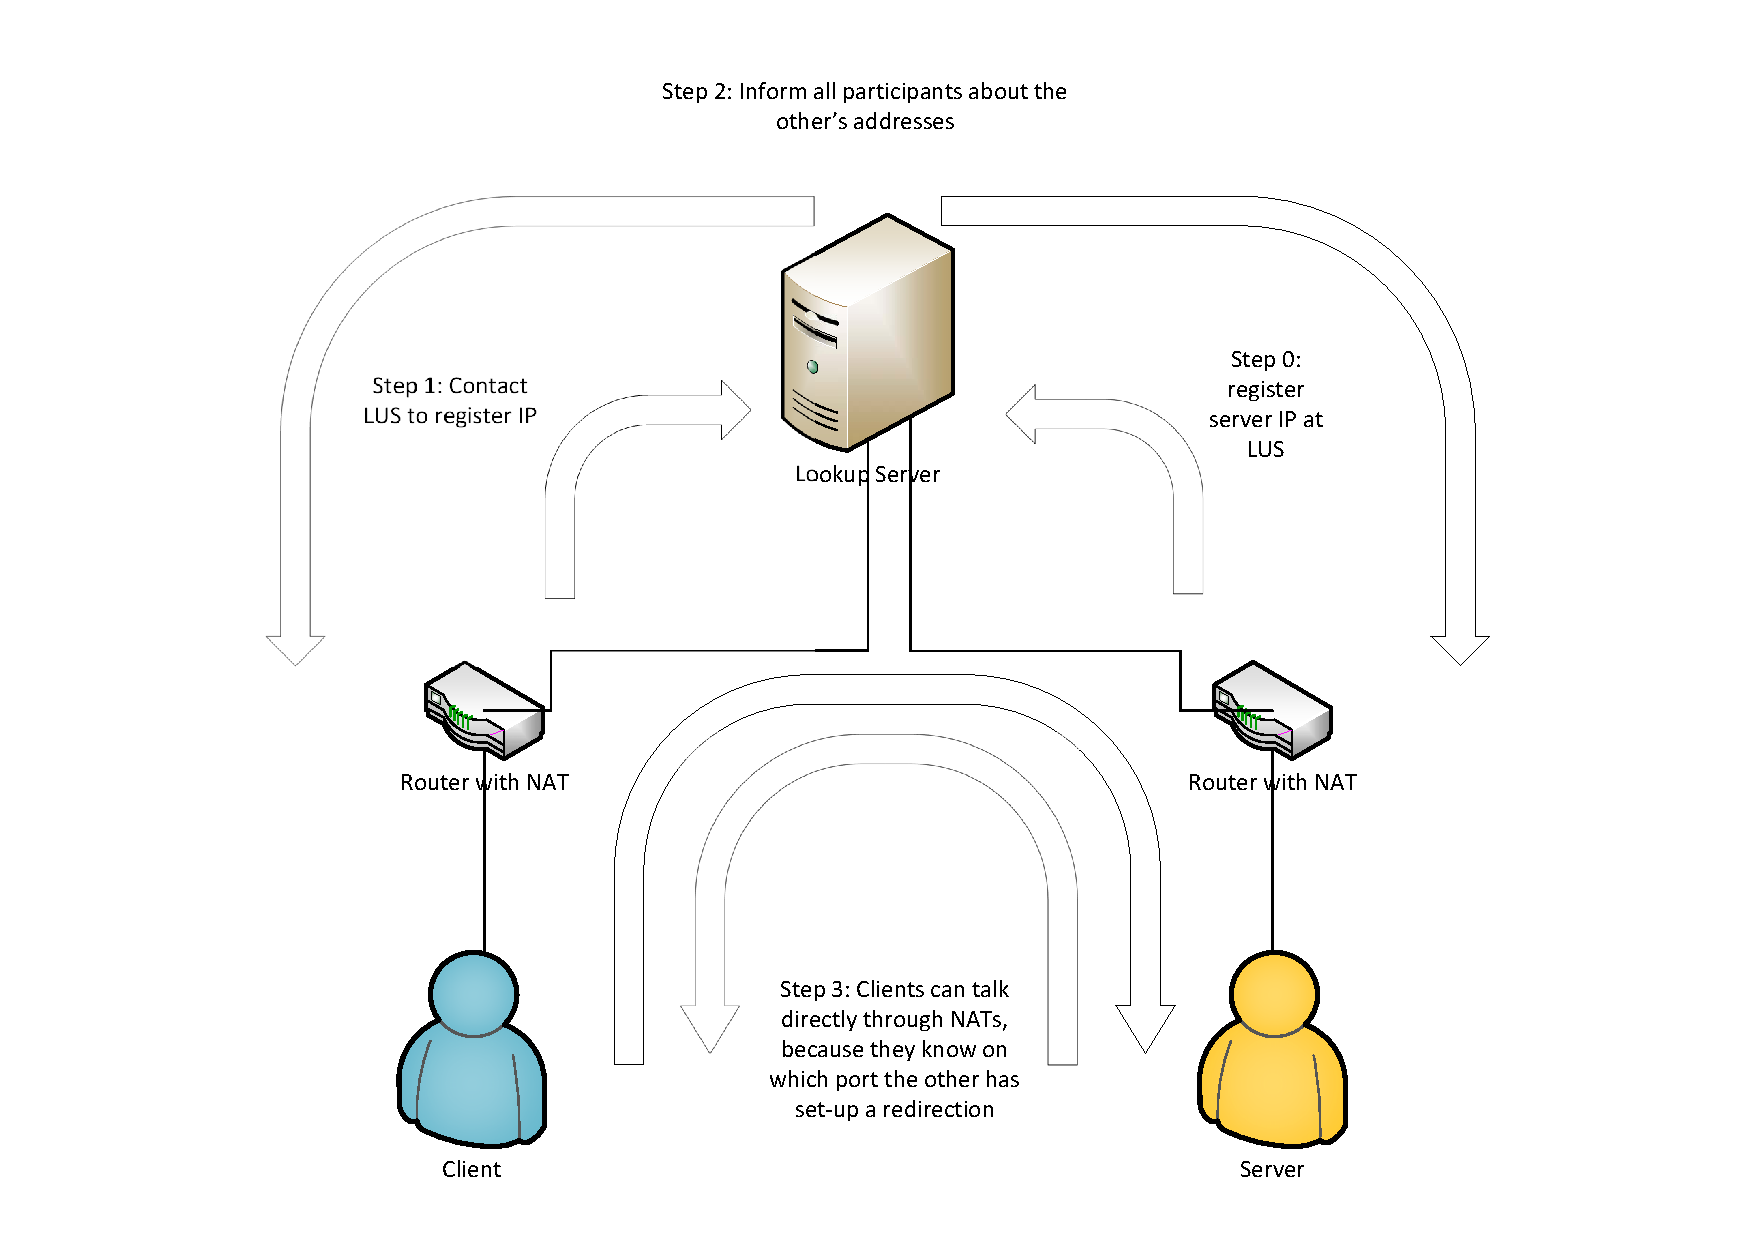
\includegraphics[width=\columnwidth]{NATholepunching.pdf}
    \vspace{-5mm} % use negative white space to fix too large gaps
	\caption{NAT-traversal}
    \lfig{nat}
\end{figure}
\subsection{DETAILED OVERVIEW}
\begin{figure}
\begin{verbatim}
{
  "header":{
    "messagegroup":"registration",
    "messagetype":"Register"
  },
  "body":{
    "username":"roger",
    "role":"player"
  }
}
\end{verbatim}
\caption{Example: Request to register user}
\lfig{regmsg}
\end{figure}

First of all, we implement a simple server-client setup and define the format and the messages that should be provided as an interface between the client and the server.(See our first~\cite{messaging} and second~\cite{messaging2} draft) At the same time, we can start implementing the user interface and writing this proposal.\\
See~\rfig{regmsg} for an example of how our messages will be structured. We encode all our messages in JSON and split them into a header which is uniform over all messages, and a body which is message-specific in content. To parse these messages, we implement factories to make the code modular.\\
That is, the \verb|ParserFactory| use the \verb|messagegroup| to create a \verb|Parser| object specific to the kind of message. Which \verb|Parser| to choose is decided via a dynamically registered mapping, which means that we can reuse the code on both the server and the client side, and that we have minimal effort if we need to change or add some type of message.\\
For example, say that we need to add a timestamp to the \verb|Register| message for some reason. Chances are that we also need to update the format of the response to this request, which for this reason has the same \verb|messagegroup|. All of this can be done by changing only the \verb|Parser| for this specific messagegroup.\\
Similarly, the \verb|Parser| instance uses an \verb|ActionFactory| and the \verb|messagetype| to actually turn the specific message into an executable method.\\
If you're interested in the most current specifications of the messages, see our github page~\cite{github}. There will at some point also be specified how we handle loss of connection, probably using our own implementation of keepalive packets.\\
\\
In a second step, once the basic communication between server and client works and the exact behaviour of the two parts has been defined, we finish implementing the serverside game logic and start using the previously defined messaging functionality.
We will make it so that the server does most of the computations and only sends the client its state, containing the players hand, the number of cards other players are holding and the most recently played cards. The client receives also a list of possible actions, from which it can choose one without having any clientside support for them, except for the user interface. This allows us to later add gamemodes and rules with ease, because we will only need to change a few classes.\\
%TODO: add state diagram?
We are also trying to keep the classes themselves very modular to make updating them - e.g. by adding further rules - just as simple.\\
Once the game is in a working state with a few rules such as an additional card like the one where the player can choose a color or the well-known "+2" card from UNO, we will decide whether we need to focus on bugfixing, cleaning up code, implementing a LUS for NAT-traversal~\rfig{nat} or adding more rule options. Adding a LUS might impose additional difficulties because some mobile carriers might use symmetric NATs. If these difficulties arise, we will probably resort to only implementing NAT-traversal for the other (easier) types of NATs.\\

We designed the User Interface for the standard scenario from starting the app to start playing to look like the following: The first screen (1) is for the player to choose, whether he wants to start a new game or join an already existing game. If he decides to start a new one, he will start the server in an android thread in the background. He will be prompted to enter his username and decide whether he wants to play or observe/spectate the game. If he presses the "Start Server" Button in (2) after filling out the missing information, he will connect himself as an admin to the previously started server running in the background of his device. After that he will be forwarded to an activity (3), with the necessary information for others to connect and a list of already connected players/observers. By pressing the settings button he will be taken to (4) and it's here where further settings and rules of the server and game can be changed. A client that joins a game will go through a similar process. He has to start by filling out his name, the host ip and port and whether he want's to act as a player or a spectator (5). Once the player connects to the server he will see a list of other players/observers, but not be able to kick them or change any settings, as this is left for the host/admin (9). When the host starts the game everyone will see the activity in which the game can be played and either see a standard view with his hand, the topmost card, all connected players and the amount of cards in each hand (6) or he will see the view of the spectator(7). Players will be able to place any by the server as placable declared card or draw cards from the heap. Spectators will see the public gamestate, but not any specific cards in any hand, they will also not be able to interact in the game. The usecase for this option, is that you could place a larger andoid device (tabled, phablet) in the middle of a table to get the "classic cardgame feel" while still playing on mobile devices. \\
\begin{figure}[h]
	\centering
    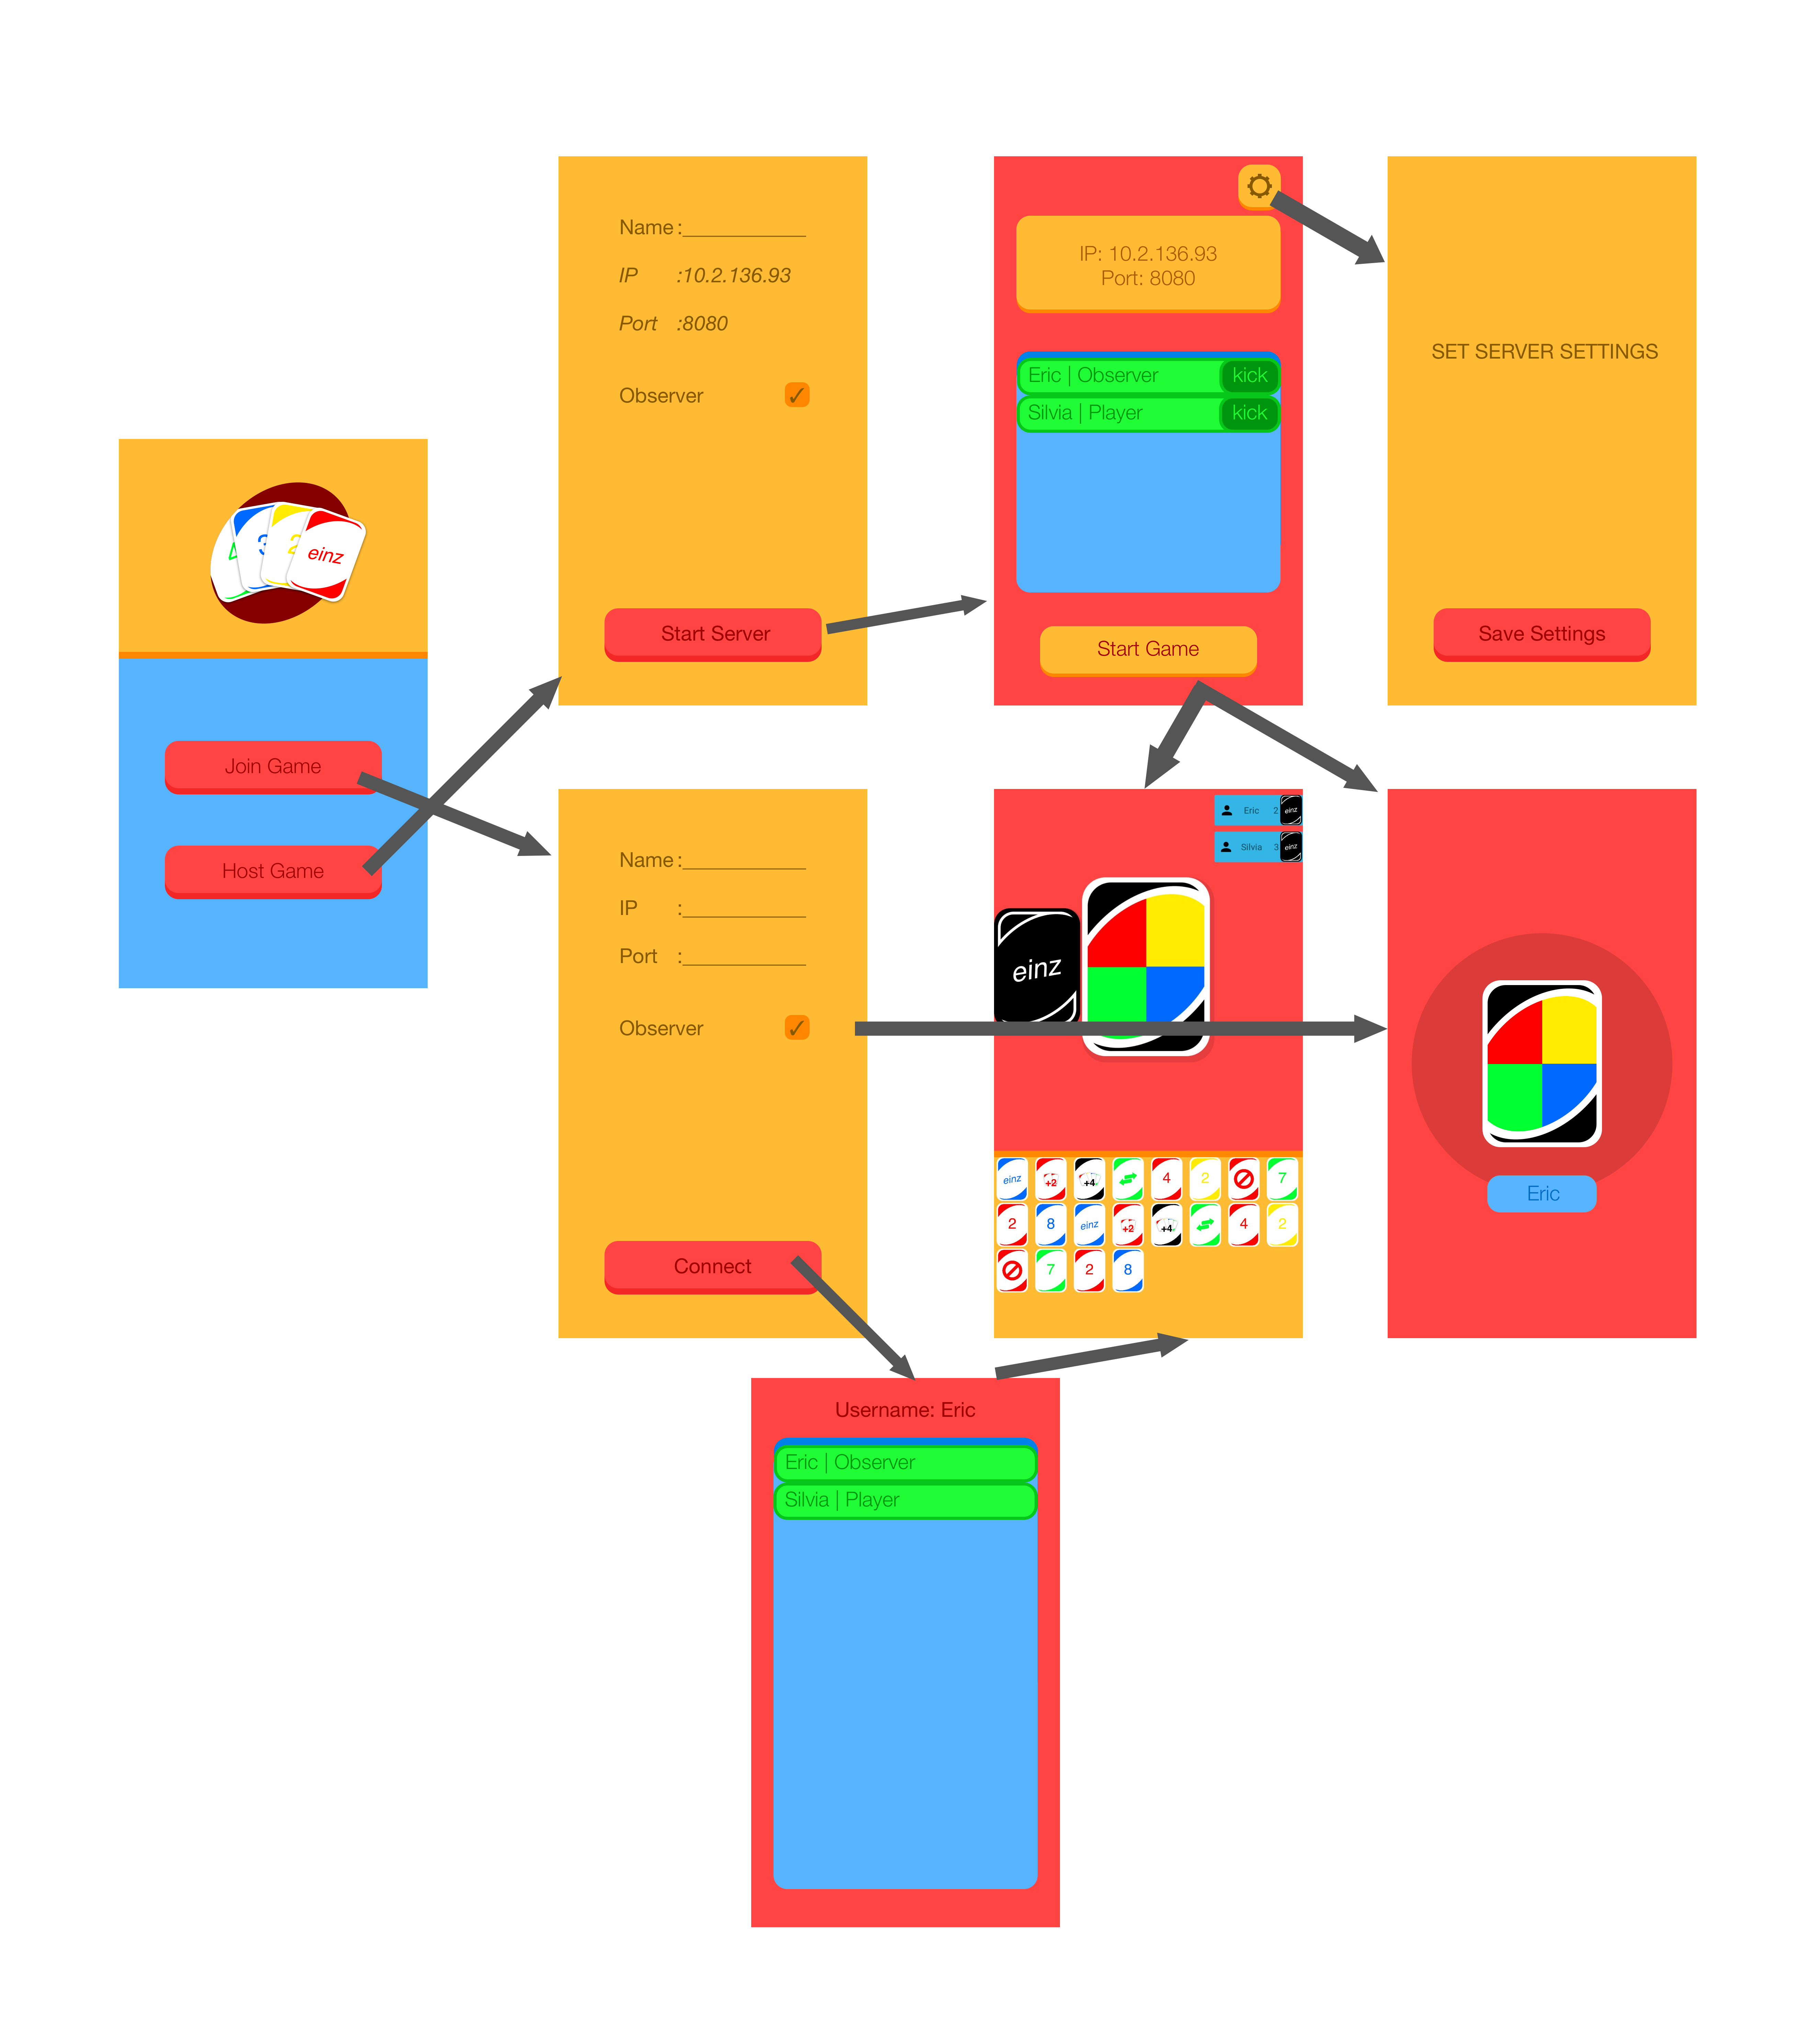
\includegraphics[width=\columnwidth]{Artboard.png}
    \lfig{nat}
    \vspace{-5mm} % use negative white space to fix too large gaps
	\caption{User Interface}
\end{figure}
\\

Regarding the difficulty of working in a larger team than most of us are used to, we intend to simplify the cooperation by using git~\cite{github} and trello~\cite{trello}. We have also appointed a Team Lead whose task it is to distribute the work so that everybody can contribute meaningfully to the Project yet also learn something while doing so.\\

To demonstrate our application in the end, we will need at least a working WiFi network and maybe internet as well, depending on how much of the NAT traversal we will have implemented.
\newline
\newline


\section{Requirements}
Our App runs on Android devices with at least Android 5.0 installed. We use the local wireless connection to communicate between the devices. One device will act as a server and waits for the clients to connect. Once every player is connected the user that started the server can start the game.


\section{Work Packages}
There work will be broken down into the following subtasks:

\begin{itemize}
        \item {\bf WP1}: Define Client-Server Communication\\
        We define the protocol that the client and the server use to communicate. Once we agreed on a message exchange protocol, the developement of the server and the client can be done separately.
        \item {\bf WP2}: Server Game Logic\\
        Implement the game logic without thinking about the networking part or multithreading
           
        \item {\bf WP3}: Client\\
	Implement functions for client to display the current state of the game according to the data received from the server and interact with the UI and the Server.
	\item {\bf WP4}: Application UI\\
	Make a UI like previously described for all the different Activities.
Add resourced for them all to have the same style.
        \item {\bf WP5}: Dynamic Message Parser\\
	Implement a reusable parsing system that maps the incoming messages to executable methods as described earlier.
        \item {\bf WP6}: Implement Client Server Protocol\\
	Register parsers and actions for every type of message specified. The server could implement this in multiple threads and has thus to call the actions in a safe way. Similarly, but single-threaded, on the client.
\end{itemize}

\section{Milestones}

\subsection{Milestone 1}
\begin{itemize}
	\item Define Client Server Protocol
\end{itemize}

\subsection{Milestone 2}
\begin{itemize}
	\item Getting client server to communicate with the Protocol
\end{itemize}

\subsection{Milestone 3}
\begin{itemize}
	\item Implement Game logic and Client UI
\end{itemize}


We think it is important to have someone who has an overview of the whole project, therefore we assigned a project manager. For the implementation of the application we made two groups, one for the server side and one for the client side. There is one person responsible for the organisation and delegation of the work to other people for both server and client side. These two people also have to set an API to make the two parts work together in the application.

As project manager and organizing the structure of the project: Josua

Server: Responsible for organisation and also helps implementing: Eric, helps with implementation: Fabian

Client: Responsible for organisation and also helps implementing: Chris, helps with implementation: Clemens

UI and Logo: Chris

First responsable for writing the proposal, then helps implementing where there is need: Silvia


% The following two commands are all you need in the
% initial runs of your .tex file to
% produce the bibliography for the citations in your paper.
\bibliographystyle{abbrv}
\bibliography{report}  % sigproc.bib is the name of the Bibliography in this case
% You must have a proper ".bib" file

%\balancecolumns % GM June 2007

\end{document}
